\documentclass{article}
\usepackage[a4paper,top=1.5cm, bottom=1.5cm, left=3cm, right=3cm]{geometry}
\usepackage[utf8]{inputenc}
\usepackage[T1,T2A]{fontenc}
\usepackage[english, russian]{babel}
\usepackage{graphicx}
\usepackage{caption}

\captionsetup[figure]{position=bottom}

\begin{document}

\begin{figure}
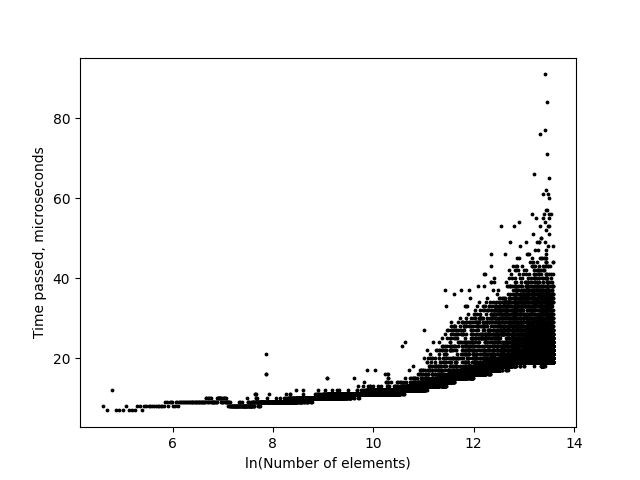
\includegraphics{average_bin.png}
\caption{Среднее время бинарного поиска}
\end{figure}

\begin{figure}
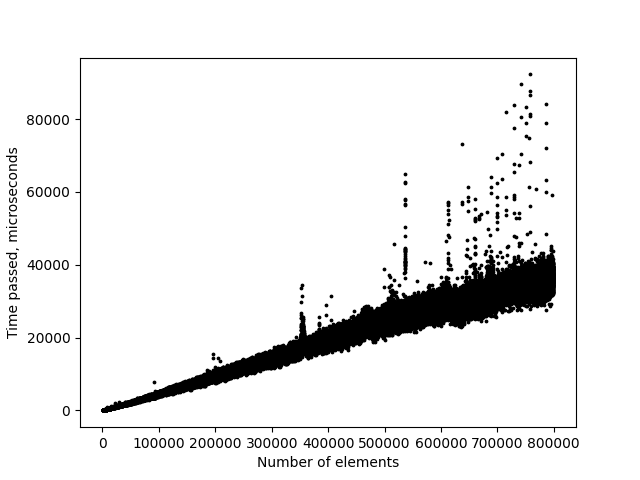
\includegraphics{average_lin.png}
\caption{Среднее время линейного поиска}
\end{figure}

\begin{figure}
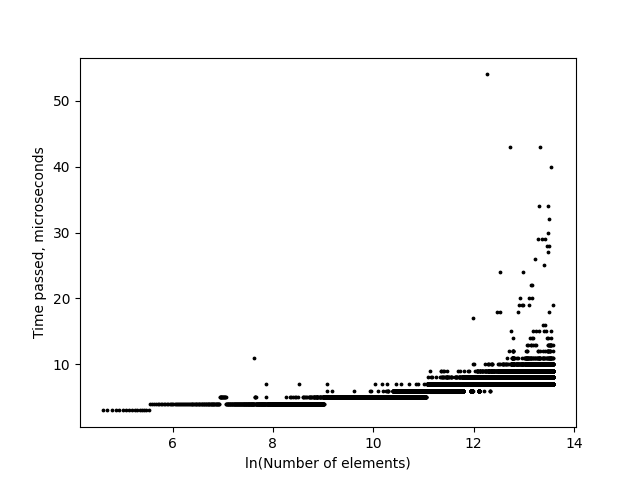
\includegraphics{worst_possible_bin.png}
\caption{Наихудшее время бинарного поиска}
\end{figure}

\begin{figure}
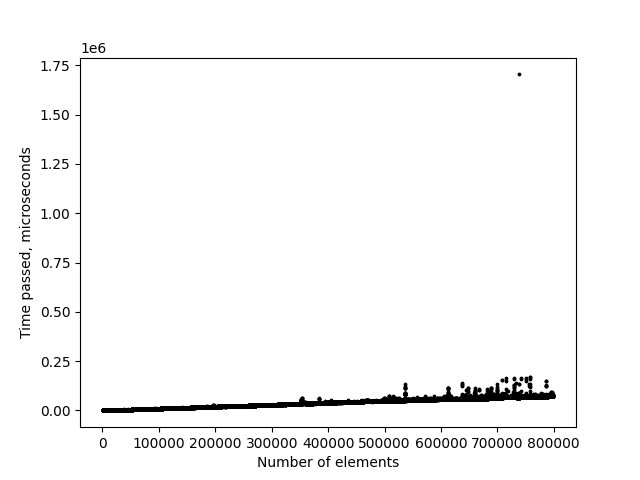
\includegraphics{worst_possible_lin.png}
\caption{Наихудшее время поиска прямым переборои}
\end{figure}

\begin{figure}
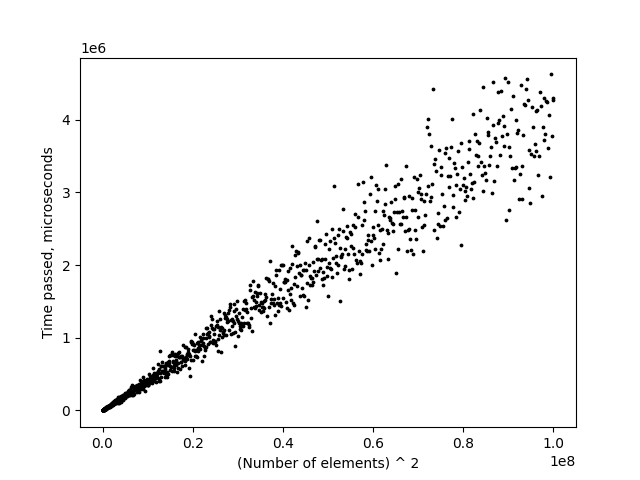
\includegraphics{quad_sum.png}
\caption{Время поиска элементов с заданной суммой в упорядоченном массиве}
\end{figure}

\begin{figure}
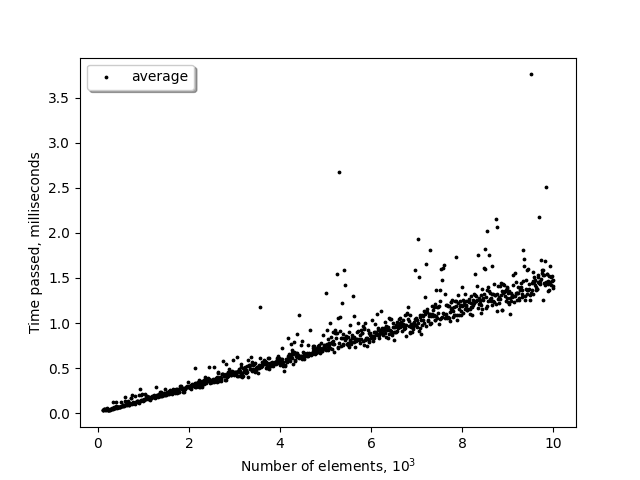
\includegraphics{lin_sum.png}
\caption{Время поиска элементов с заданной суммой полным перебором}
\end{figure}

\begin{figure}
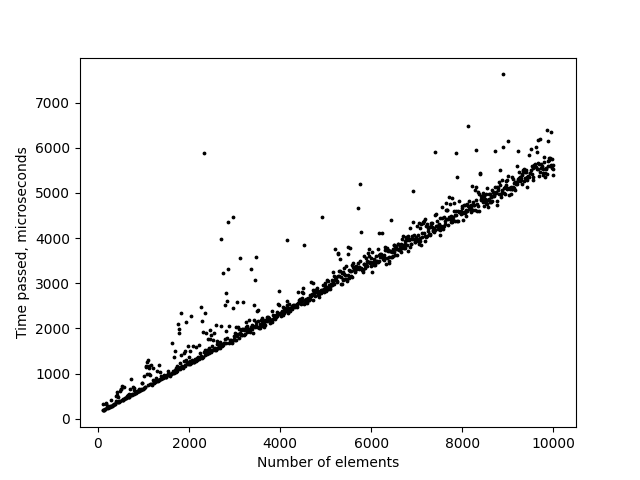
\includegraphics{A_uniform.png}
\caption{Время поиска равномерно распределенных запрсов при использовании стратегии A}
\end{figure}

\begin{figure}
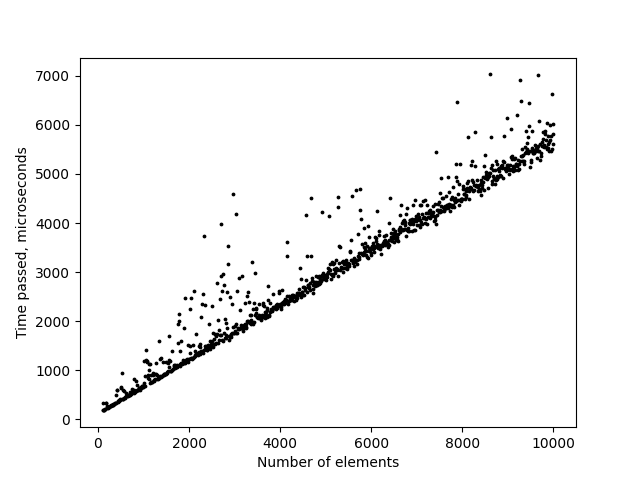
\includegraphics{B_uniform.png}
\caption{Время поиска равномерно распределенных запрсов при использовании стратегии B}
\end{figure}

\begin{figure}
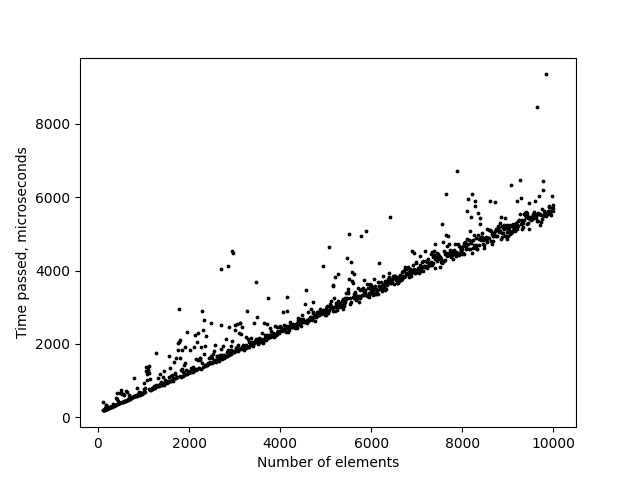
\includegraphics{C_uniform.png}
\caption{Время поиска равномерно распределенных запрсов при использовании стратегии C}
\end{figure}

\begin{figure}
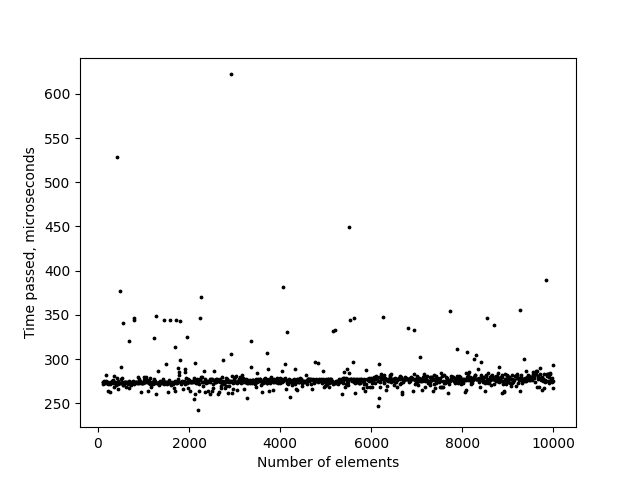
\includegraphics{A_binomial.png}
\caption{Время поиска биномиально распределенных запрсов при использовании стратегии A}
\end{figure}

\begin{figure}
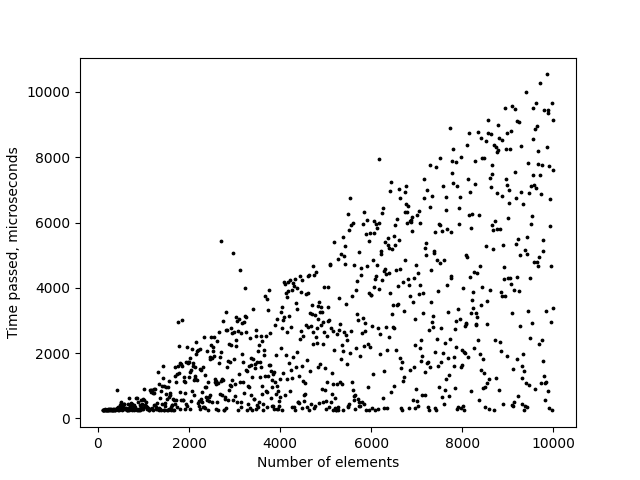
\includegraphics{B_binomial.png}
\caption{Время поиска биномиально распределенных запрсов при использовании стратегии B}
\end{figure}


\begin{figure}
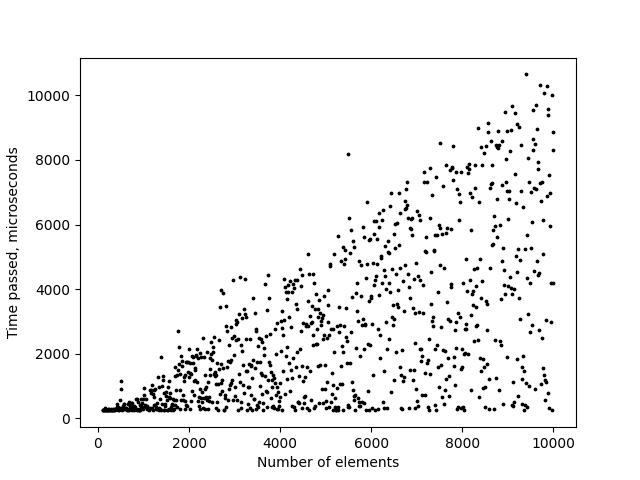
\includegraphics{C_binomial.png}
\caption{Время поиска биномиально распределенных запрсов при использовании стратегии C}
\end{figure}


\end{document}